\chapter{Experiments}
\label{Experiments}
\overridetextsize

\section{Overview}
\label{sec:experiments_overview}


Adversarial examples can be seen as a worst-case noise that fools the model into
misclassification when applied to an image. On the other hand, neural networks
are relatively robust to random corruptions such as Gaussian noise.

My intuition is that applying random noise to an adversarial example could hide
or alter parts of the adversarial perturbation, thus diminishing or even
nullifying its effect.

In order to apply a random transformation to an image $x$, we generate a
Gaussian noise $\tilde{y}=\mathcal{N}(0,1)$ that we add to the image in order to
create a noisy version $\tilde{x}$:
\begin{align} \label{eq:noisy_version}
    \tilde{x}=x+\tilde{y}\kappa,
\end{align}
where $\kappa$, is the standard deviation used to scale down or up the noise
intensity.

\begin{figure}
    \subfloat[]{%
        \includegraphics[clip,width=.33\linewidth]{Figures/noise/std:0.0,l2:
            0.0,PSNR:100.0.png}%
    } \subfloat[]{%
        \includegraphics[clip,width=.33\linewidth]{Figures/noise/std:0.02,l2:
            5.1,PSNR:34.01.png}%
    } \subfloat[]{%
        \includegraphics[clip,width=.33\linewidth]{Figures/noise/std:0.04,l2:
            10.13,PSNR:28.05.png}%
    }

    \subfloat[]{%
        \includegraphics[clip,width=.33\linewidth]{Figures/noise/std:0.06,l2:
            15.07,PSNR:24.6.png}%
    } \subfloat[]{%
        \includegraphics[clip,width=.33\linewidth]{Figures/noise/std:0.08,l2:
            19.91,PSNR:22.18.png}%
    } \subfloat[]{%
        \includegraphics[clip,width=.33\linewidth]{Figures/noise/std:0.1,l2:
            24.61,PSNR:20.34.png}%
    }

    \caption{ Increasing the noise intensity $k$ on an ImageNet sample. Details
        in Table \ref{table:noise_increase}.}
    \label{fig:noise_increase}
\end{figure}

Fig \ref{fig:noise_increase} shows the impact of increasing $\kappa$ on an image
and shows the corresponding $L_2$ distance and peak signal-to-noise ratio (PSNR)
of the noise mask.

\begin{table}[htb]
    \centering
    \begin{tabular}{c c c c}
        \toprule
        Image & $k$  & $L_{2}$ & PSNR  \\
        \midrule
        A     & 0.00 & 0.00    & 100   \\
        B     & 0.02 & 7.76    & 34.01 \\
        C     & 0.04 & 15.46   & 28.05 \\
        D     & 0.06 & 23.11   & 24.60 \\
        E     & 0.08 & 30.40   & 22.18 \\
        F     & 0.10 & 37.36   & 20.34 \\
        \bottomrule
    \end{tabular}
    \caption{Details for Figure \ref{fig:noise_increase}}
    \label{table:noise_increase}
\end{table}

To further motivate and formulate the proposed method discussed in section
\ref{Methodology}, I first perform a series of experiments detailed in the
remainder of this section to verify that the intuition mentioned above holds
correct.

\section{Experimental Settings}
Below I describe the datasets and models used, as well as the settings used to
configure the attack methods.

\subsection{Datasets and Models}
\label{sub:datasets_models}

To conduct the experiments, I collect data from three datasets:
\begin{itemize}
    \item CIFAR-10 \cite{krizhevsky_learning_2009}, widely used dataset
          consisting of 60000 $32 \times 32$ RGB images divided into ten
          different classes (e.g., airplane, automobile, bird.). For the
          experiments, I use the 10.000 images present in the test set.
    \item ImageNet \cite{russakovsky_imagenet_2015}, popular image database
          containing over 1.300.000 $224 \times 224$ RGB images divided into
          1000 different classes. For our experiments, rather than using the
          entirety of the dataset, I created a subset containing 10 of ImageNet
          classes.
    \item Dogs vs. Cats \cite{elson_asirra_2007}, the Asirra (Animal Species
          Image Recognition for Restricting Access) is a real-world Kaggle
          dataset containing 25.000 $224 \times 224$ resized RGB images divided
          into two classes: dogs and cats.
\end{itemize}

For the models, we use a Very Deep Convolutional Networks for Large-Scale Image
Recognition with 11 layers \cite{simonyan_very_2015-2}. The
complete architecture of the VGG-11 model is shown in table \ref{table:vgg11}.

\begin{table}[htb]
    \centering
    \begin{tabular}{c c}
        \toprule
           & VGG 11             \\
           & Input (224x224x3)  \\
        \midrule
        1  & Conv. 64           \\
           & Maxpool            \\
        \hline
        2  & Conv. 128          \\
           & Maxpool            \\
        \hline
        3  & Conv. 256          \\
        4  & Conv. 256          \\
           & Maxpool            \\
        \hline
        5  & Conv. 512          \\
        6  & Conv. 512          \\
           & Maxpool            \\
        \hline
        7  & Conv. 512          \\
        8  & Conv. 512          \\
           & Maxpool            \\
        \hline
        9  & FC 4096            \\
        10 & FC 4096            \\
        11 & FC 1000 ($\sigma$) \\
        \bottomrule
    \end{tabular}
    \caption{VGG configuration with 11 layers}
    \label{table:vgg11}
\end{table}

We use pre-trained on ImageNet models open-sourced by PyTorch for the
experiments using the ImageNet and Dogs vs. Cats datasets. For Dogs vs. Cats,
the model is fined-tuned, \emph{i.e.,} the last few layers' parameters are
updated instead of training the whole network from scratch.

\subsection{Attacks}
\label{sec:attack}
I implement the attacking methods introduced in Section
\ref{Adversarial_examples} using the FoolBox library \cite{rauber_foolbox_2020}.
For targeted attacks defined in section \ref{Adversarial_examples}, the target
$t$ class is selected randomly such that
\begin{align} \label{eq:targeted}
    \left\{ t:t\in C \backslash \left\{
    y\right\}\right\},
\end{align}
where $C$ is a set of the available classes in the dataset and $y$ is the
ground-truth label of the sample.

I generate adversarial examples using accurately classified images from the test
sets of each dataset as it would not make sense generating adversarial examples
on samples that the models already fail to identify.

\section{Robustness}
\label{sec:robustness}

In this section, in order to verify the intuition mentioned in section
\ref{sec:experiments_overview}, I describe two experiments where I apply noise
to both the input images and the adversarial examples in order to compare the
model's output before and after the added noise.


\subsection{Consistency}
\label{sub:consistency}

\begin{figure}[htp]
    \subfloat[]{%
        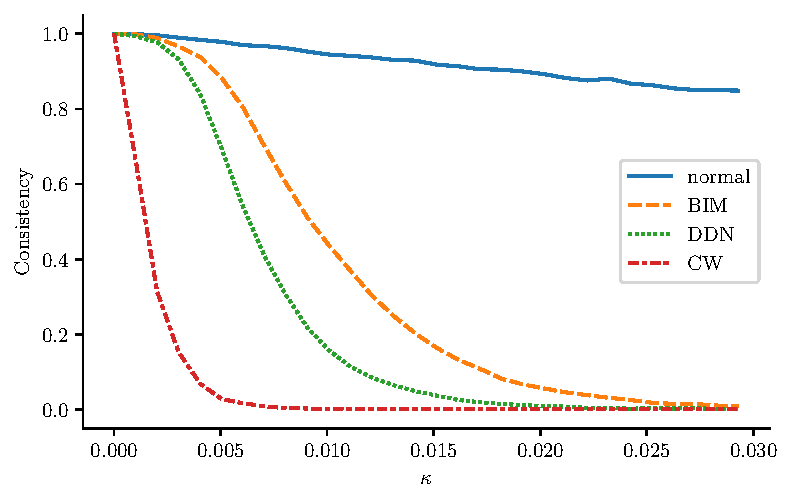
\includegraphics[clip,width=\columnwidth]{figures/fig2a.pdf}%
    }

    \subfloat[]{%
        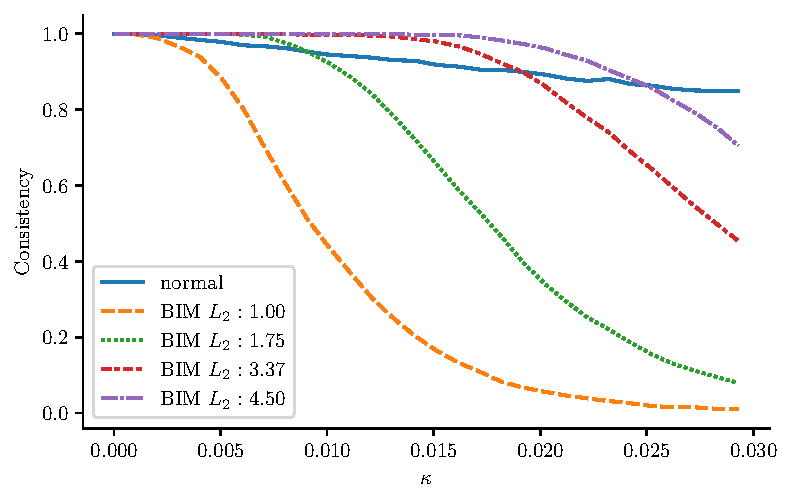
\includegraphics[clip,width=\columnwidth]{figures/fig2b.pdf}%
    }

    \caption{Consistency comparison between normal images and adversarial
        examples using different methods and perturbation budgets. As $\kappa$
        (see \eqref{eq:noisy_version}) increases, the consistency decreases,
        more so for adversarial examples, unless we also increase the
        adversarial perturbation budget as seen in (b).}
    \label{fig:consistency}
\end{figure}


In the first experiment, I compare the model's classification output for a
normal image $x$ and a transformed version $\tilde{x}$ (Eq.
\eqref{eq:noisy_version}). When the classifications $C(x)$ and $C(\tilde{x})$
are identical, I refer to them as being \emph{consistent} classifications.
\emph{i.e.,} when the model predicts the same class for the unperturbed image
and the same image but containing voluntarily added noise, the predictions are
consistent with one other. If my intuition is correct, we should observe the
predictions on normal images to be more consistent when adding noise. At the
same time, I expect the model's predictions on adversarial examples to start
being more inconsistent as the noise intensity increases.

Here, our objective is to compare the consistency between normal images and
adversarial examples. To proceed, I randomly select 1000 images from ImageNet's
test set to record the classification consistency on each sample and at
different $\kappa$ (Eq. \eqref{eq:noisy_version}) values. Finally, we follow the
same procedure for adversarial examples and generate 1000 samples with the BIM,
DDN, and CW methods.

Figure \ref{fig:consistency} shows the average classification consistency of
input types and at different $\kappa$. We observe the average consistency to
decrease slowly as $\kappa$ increases for normal images. This moderate decrease
shows that, as expected, the model is not significantly affected by the random
perturbation added to the image. On the contrary, we observe that adversarial
examples' classification consistency decreases rapidly as $\kappa$ increases.
These results corroborate my intuition that introducing random perturbations to
an adversarial example could impede its effectiveness.

\begin{figure}[ht]
    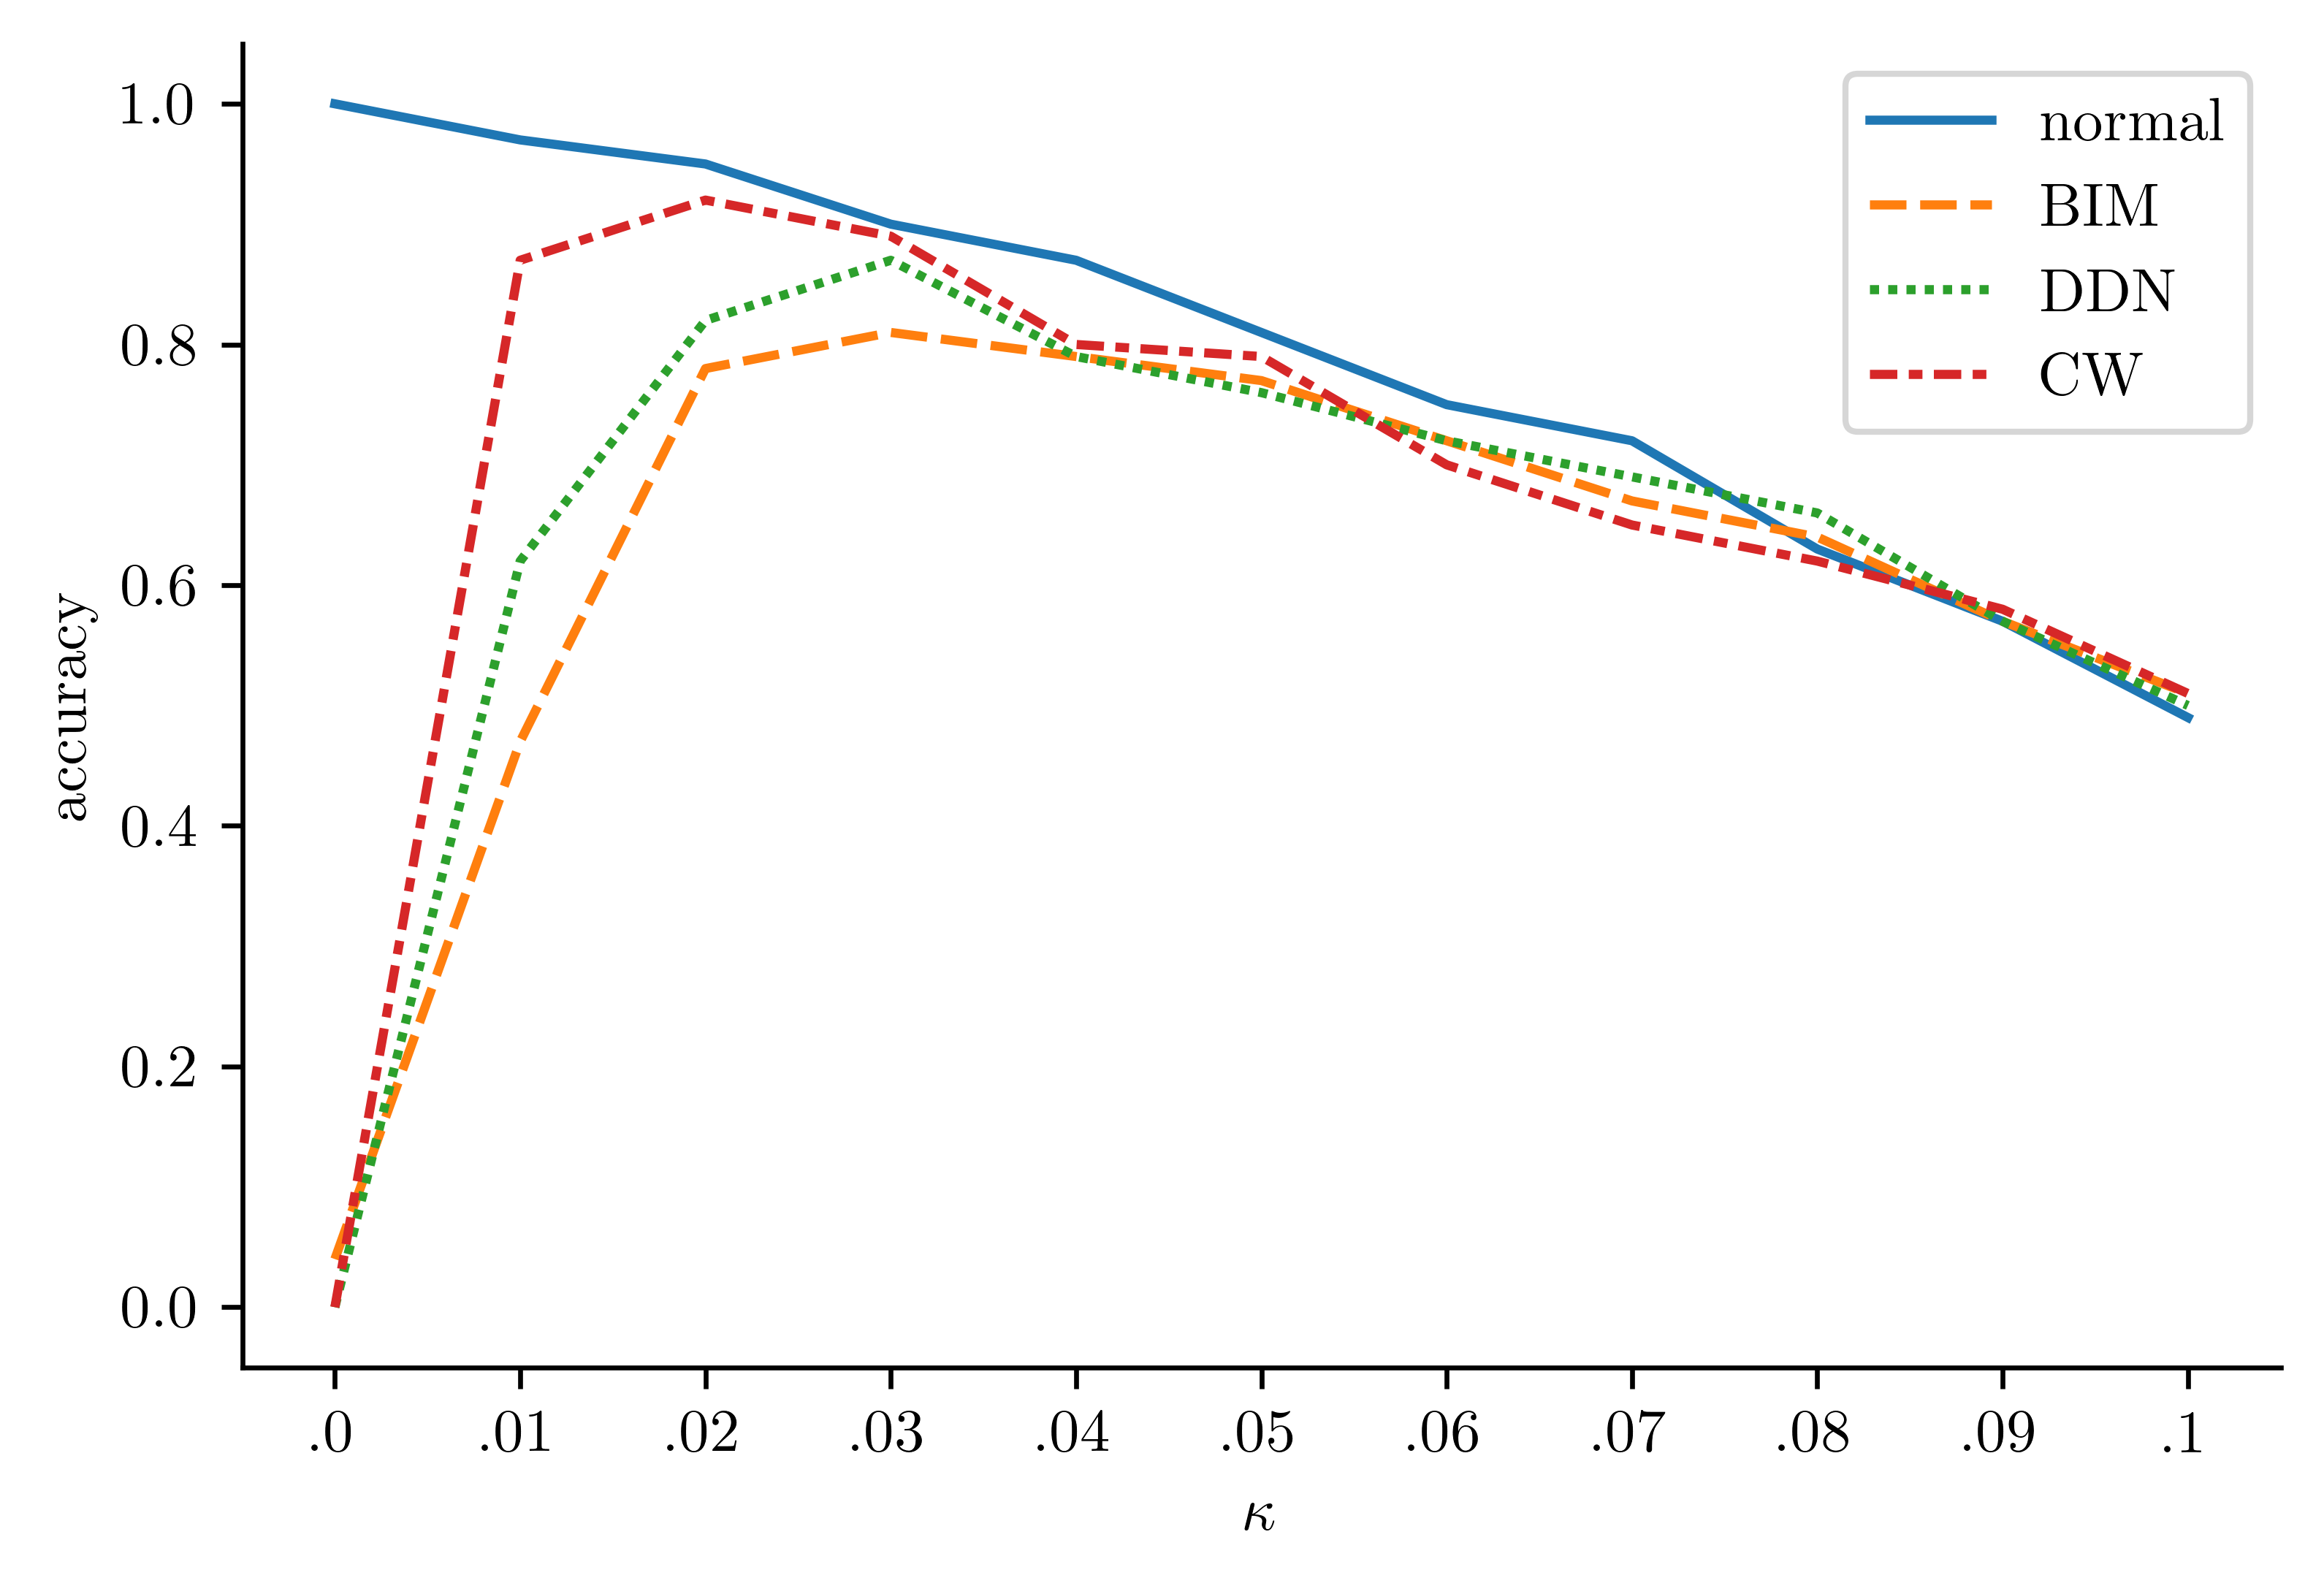
\includegraphics[width=\columnwidth]{Figures/experiments/accuracy.png}%
    \caption{Shows the accuracy comparison between normal images and adversarial
        examples; as $\kappa$ increases, the accuracy of adversarial examples first
        increases before decreasing similarly to normal images.}
    \label{fig:accuracies}
\end{figure}

Furthermore, figure \ref{fig:accuracies} shows that the actual prediction
accuracies are partially restored on adversarial examples as the noise intensity
increases before slowly reducing again, similarly to normal images, when the
noise intensity is too high for the model. Finally, average accuracies of normal
images and adversarial examples start to be very similar at around $0.03
    \kappa$, hinting and showing again that the adversarial perturbations in
adversarial examples lost their efficacy to fool the targeted models.


Interestingly, coming back to figure \ref{fig:consistency}A, we can also observe
the classification consistency being different between attacking methods,
\emph{i.e.,} to reach a consistency of $\approx 0$, adversarial examples
generated with BIM need a larger $\kappa$ than samples generated with DDN and
CW.

Instinctively, this difference makes sense; adversarial examples generated with
the BIM approach have a larger average $L_2$ adversarial perturbation of
$\approx 1.0$ compared with DDN at $L_2\approx0.85$ and CW at $L_2\approx0.70$.
Figure \ref{fig:consistency}b shows the same experiment but using adversarial
examples generated with BIM at different perturbation budgets. These results
undeniably show that the more substantial the adversarial perturbation is
(\emph{i.e.,} higher perturbation budget), the more robust it is to random
perturbations. Therefore, a larger $\kappa$ may be needed to counter the
effectiveness of the higher adversarial perturbation budget attacks.

\subsection{Logits differences}
\label{sub:logits_differences}
\begin{figure}[ht]
    \centering
    \subfloat[Normal Image]{%
        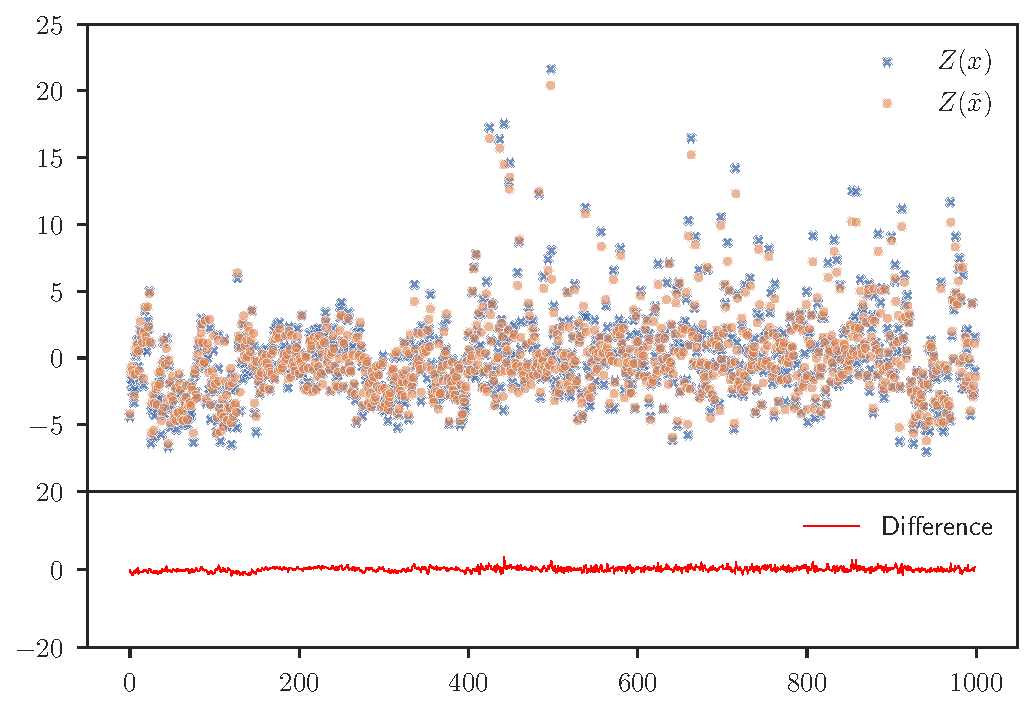
\includegraphics[clip,width=0.9\columnwidth]{figures/fig4a.pdf}%
    }

    \subfloat[Adversarial Example (BIM)]{%
        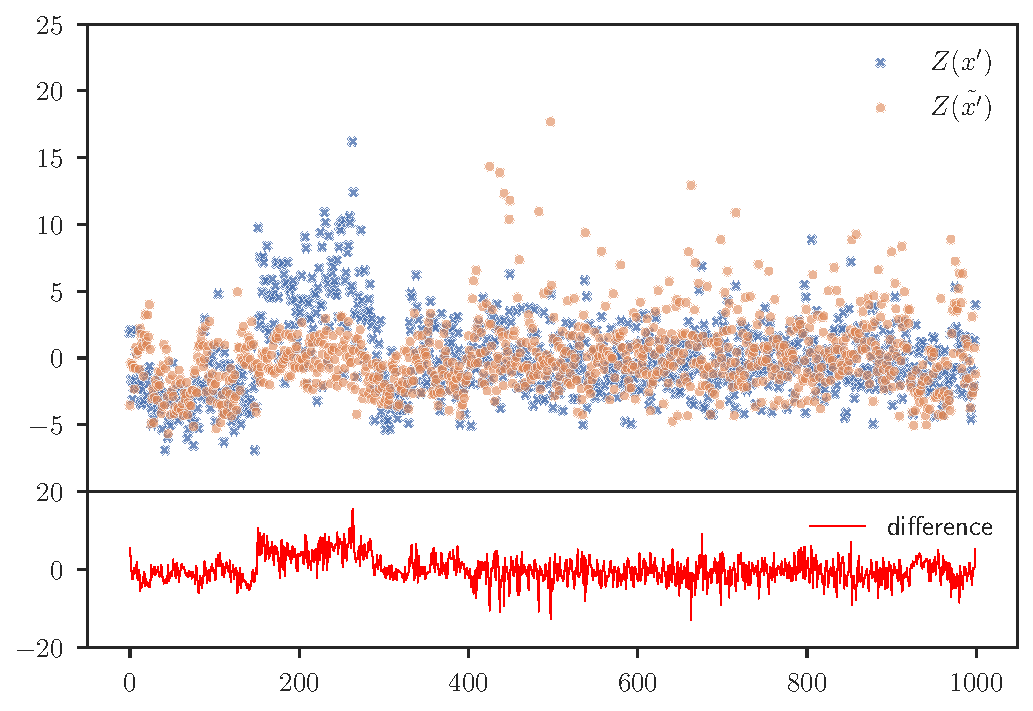
\includegraphics[clip,width=0.9\columnwidth]{figures/fig4b.pdf}%
    } \caption{Comparison between the logits of an ImageNet image before
        ($Z(x)$) and after adding noise to the input ($Z(\tilde{x})$). When the
        input is normal (A), the difference between predictions is small, but
        becomes larger when the input is adversarial (B).}
    \label{fig:logits}
\end{figure}

I performed another experiment to investigate further the difference between the
model output for an untransformed and a randomly perturbed image. Instead of
recording the classification output of the model as done in section
\ref{sub:consistency}, which is only a reduced-down portion of the output, I
decided to observe the output logits, \emph{i.e.,} the output before applying
the activation function: in this case, before applying softmax. This will allow
us to see the raw output values for each class.

I select a single ImageNet image $x$ and generate a noisy version $\tilde{x}$
with $\kappa=\num{2e-2}$. Figure \ref{fig:logits}A shows the output logits
$Z(x)$ and $Z(\tilde{x})$ for each the normal image $x$ and the perturbed
version $\tilde{x}$ respectively. Logits are plotted (1000 logits for the 1000
ImageNet classes), as well as the difference between $Z(x)_i$ and
$Z(\tilde{x})_i$ in the lower part of the plot. We observe both outputs to be
very similar value-wise for each class. On the contrary, when the original input
is adversarial (BIM, $L_2 \approx 1$), as in figure \ref{fig:logits}B, the
difference between outputs is striking, magnitudes over the difference observed
with the normal image.

These two experiments proved that my initial intuition was correct. It also
showed that the higher budget the adversarial perturbation, the more robust it
is against the random perturbation I add to the input. To me, this may explain
why many detection techniques fail to detect higher-perturbation budgets
adversarial examples. These observations motivated me to pursue this track
because I believe that the ease with which we can add varying random
perturbation to the input, by increasing or decreasing $\kappa$, could be an
interesting idea to combat low \emph{and} high perturbation budgets attacks.

Observing and comparing the model outputs showed us that adding a random
perturbation to an image can help us detect the legitimate or adversarial nature
of the input.

Following these observations, I present in the following section a novel method
to detect adversarial examples.
